% CALC16b
% Exploited Nicolini BH2-Pruefung Beamer Classes Sven
%
% um Handout=kurze Version ohne Interactive
% zu machen, folgende Zeile nutzen:
%\documentclass[xcolor=dvipsnames,handout]{beamer}
\documentclass[xcolor=dvipsnames]{beamer}
\usepackage{tikz}
\usepackage[utf8]{inputenc}
\usepackage{hyperref}
\usepackage{amsmath}
\usepackage{cite}
\usepackage{units} % nicefrac
\usepackage{datetime} % fuer Uhrzeit im \date
\usepackage{wrapfig} % bilder rechts
\usepackage{caption} % fuer subcaption
\usepackage{subcaption} % subfigures
\usepackage{booktabs} % tables
\usepackage{mathtools} % right cases
\usepackage{color}

% Schriften
% Palatino for rm and math | Helvetica for ss | Courier for tt


%%\usepackage{mathpazo} % math & rm
%%\linespread{1.05}        % Palatino needs more leading (space between lines)
%%\usepackage[scaled]{helvet} % ss
%%\usepackage{courier} % tt
%%\normalfont
%%\usepackage[T1]{fontenc}

% Hyperref aufsetzen
\hypersetup{
    pdftitle={Sven Köppel 2nd Talk Journal Club Quantum Gravity FIAS Frankfurt 25. Jun 2014},
    pdfauthor={Sven Köppel},
    pdfsubject={fias},
    pdfkeywords={physik} {black holes} {uni} {frankfurt},
    colorlinks=false,        % test: stat gerahmten Links
    linkcolor=red,          % color of internal links
    citecolor=darkgreen,    % color of links to bibliography
    filecolor=darkred,      % color of file links
    urlcolor=cyan           % color of external links
}

% Allgemeine Meta-Daten, genutzt fuer titlepage
\title{Holographic and self-encoding regular Black~Holes}
\subtitle{my Master's project}
\institute{Institut für theoretische Physik \\ Frankfurt Institute for Advanced Sciences \\ Goethe-Universität Frankfurt}
\author{\href{https://fias.uni-frankfurt.de/~koeppel}{Sven Köppel}\\
\small \texttt{koeppel@fias.uni-frankfurt.de}}
\date{Journal Club in High Energy Physics \\ Wed. 25. Jun 2014  \\ \gray \small Calc-16b} %\today, \currenttime}

% Beamerclasses theme waehlen

\usetheme[compress]{Singapore}
\usecolortheme{orchid}
%\usetheme[compress]{fiasbeamer/beamerthemefias}

% KLAPPT NICHT: 
%\usepackage{tikz}
%\usetikzlibrary{calc}
%\usetheme{fias}

\setbeamertemplate{footline}[frame number]
\beamertemplatenavigationsymbolsempty

% Hack um Subtitles als Frametitles zu nutzen,
% Bulletpoint fuer jede slide

\addtobeamertemplate{frametitle}{\let\insertframetitle\insertsubsectionhead}{}
\makeatletter
  \CheckCommand*\beamer@checkframetitle{\@ifnextchar\bgroup\beamer@inlineframetitle{}}
  \renewcommand*\beamer@checkframetitle{\global\let\beamer@frametitle\relax\@ifnextchar\bgroup\beamer@inlineframetitle{}}
\makeatother

% Beamer: Weniger Abstand zwischen Formeln!
\expandafter\def\expandafter\normalsize\expandafter{%
    \normalsize
    \setlength\abovedisplayskip{3pt}
    \setlength\belowdisplayskip{3pt}
    \setlength\abovedisplayshortskip{3pt}
    \setlength\belowdisplayshortskip{3pt}
}


% abgefahrenes highlighting von formeln
\usepackage{xcolor}
% klappt net, was einfacheres:
\newcommand{\highlight}[1]{%
  \colorbox{green!30}{$\displaystyle#1$}}


% MATH
\renewcommand{\d}{\mathrm{d}}
\newcommand{\dd}[2]{\frac{\mathrm{d} #1}{\mathrm{d} #2}}
\newcommand{\pp}[2]{\frac{\partial #1}{\partial #2}}
\renewcommand{\L}{L_P}
\newcommand{\pr}{p_r}
\newcommand{\psenk}{p_\perp}
\newcommand{\ebenso}{\biggl( ~ \therefore ~ \biggr) }
\newcommand{\metrik}[1]{\d s^2 = \left( #1 \right) \d t^2 \left( #1 \right)^{-1} \d r^2 + r^2 \d \Omega_{D-2}^2 }
\newcommand{\winkel}{r^2 \d \Omega^2}
\newcommand{\dann}{$\rightarrow~$}
\newcommand{\CA}{ {\cal A}}
\newcommand{\C}[1]{ {\cal #1}}
\newcommand{\mn}{_{\mu\nu}}

% colored symbols:
% http://tex.stackexchange.com/questions/85033/colored-symbols
\newcommand*{\mathcolor}{}
\def\mathcolor#1#{\mathcoloraux{#1}}
\newcommand*{\mathcoloraux}[3]{%
  \protect\leavevmode
  \begingroup
    \color#1{#2}#3%
  \endgroup
}
% In Text: $a\textcolor{red}{\ast}b$
% In Math: $a\mathcolor{red}{\ast}b$
\newcommand{\redmin}{\mathcolor{red}{-}}
\newcommand{\redplus}{\mathcolor{red}{+}}
\newcommand{\pn}{\mathcolor{red}{+ n}}
\newcommand{\n}{ {\mathcolor{red}{n}} }

% Gray out parts in equations
\newcommand{\gray}{ \color{gray} }
\newcommand{\black}{ \color{black} }

% Gelbe box ohne Extraplatz
% http://tex.stackexchange.com/questions/23681/colorboxcolortext-without-increasing-the-height-and-width-of-the-cell-in-a
\newcommand{\gelb}[1]{ {\setlength{\fboxsep}{0pt}\colorbox{yellow}{$#1$}} }
\newcommand{\green}[1]{ {\setlength{\fboxsep}{0pt}\colorbox{green}{$#1$}} }
\newcommand{\plus}{\gelb{+}}
\newcommand{\minus}{\green{-}}
\newcommand{\even}{\mathcolor{Violet}{even}}
\newcommand{\odd}{\mathcolor{Violet}{odd}}

% placeholder chars
\newcommand{\bul}[1]{ {\mathord{\color{#1!55}\bullet}} }

% Referenzen auf Listen...
\newcommand*\kugel[1]{\tikz[baseline=(char.base)]{
            \node[shape=circle,inner sep=2pt,fill=blue!70, text=white] (char) {\scriptsize #1};}}

% Colors of plot
\definecolor{MathYellow}{RGB}{170, 170, 0}
\definecolor{MathMagenta}{RGB}{170, 0, 170}
\definecolor{MathBlue}{RGB}{230,230,255}

\begin{document}

\frame{\titlepage} 

%\frame{\frametitle{Inhaltsverzeichnis}\tableofcontents} 

\section{Introducion}
\subsection{The holy grail}
\begin{frame}
\begin{picture}(320,250)
\put(8,20){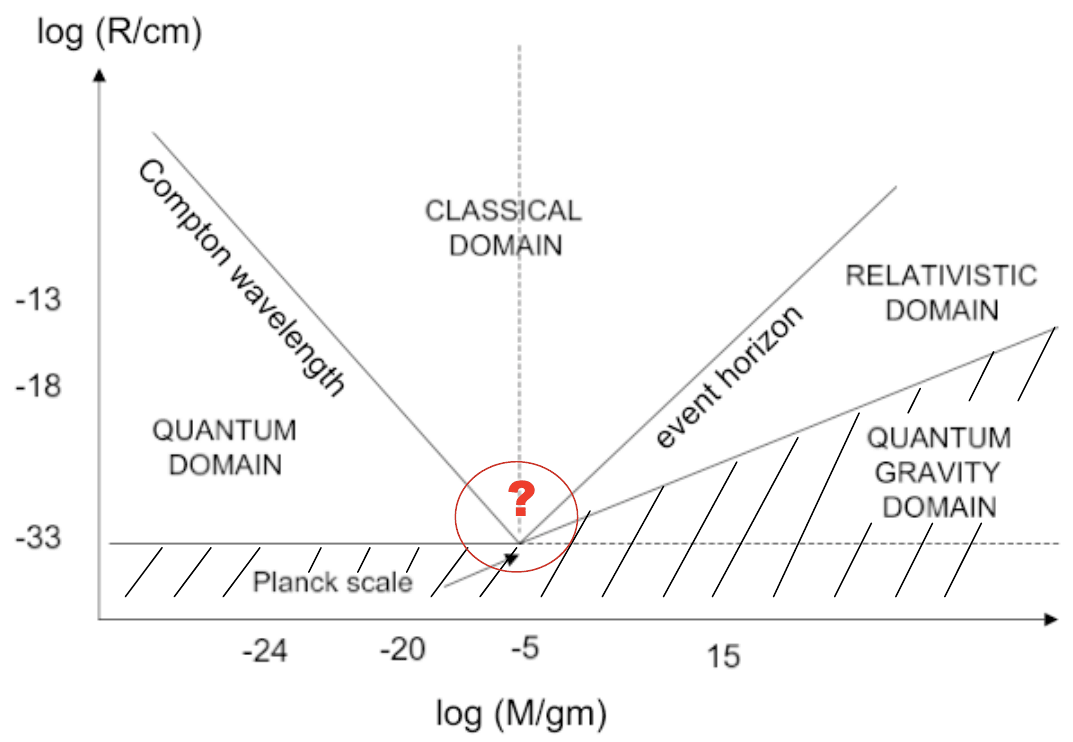
\includegraphics[width=0.8\paperwidth]{pics/Carr-Feb2014.png}}
\put(-20,20){\tiny \textcolor{gray}{Source: Carr@KSM Frankfurt 2013  arXiv:1402.1427}}
\end{picture}
\end{frame}

\subsection{A wishlist}
\begin{frame}
\begin{picture}(320,250)
\put(-8,238){\begin{minipage}[t]{0.5\linewidth}
\setbeamertemplate{enumerate items}[circle] 
\begin{enumerate}
\item Regular {\gray(No curvature singularity at origin)}
\begin{equation*}
\gray \lim \limits_{r\to 0}~ g_{00}(r) < \infty
\end{equation*}
\item Classical Limit {\gray (Schwarzschild)}
\begin{equation*}
\gray g_{00}(r) = \frac{2 G m}{r} ~~\text{for}~~ r > l_0
\end{equation*}
\item Self-encoding. $\gray r_0 = l_0$
\end{enumerate}
\end{minipage}}
\pause
\put(150,100){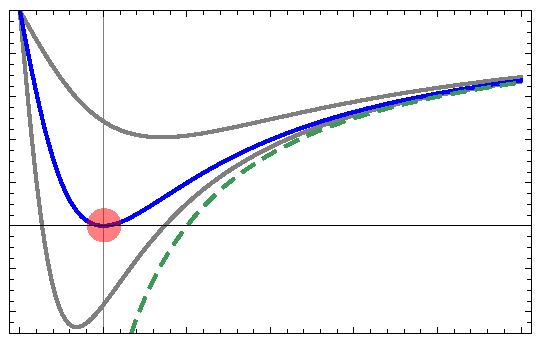
\includegraphics[width=6cm]{pics/remnant-plot-Calc07.pdf}}
\put(150,220){\small $\downarrow$ \textcolor{gray}{Generic $g_{00}$ that fulfills all requirements.}}
\pause
\put(40,98){\begin{minipage}[t]{0.8\linewidth}
\setbeamertemplate{itemize items}[circle]
\setbeamercolor{itemize item}{fg=gray}
\begin{block}{Metric candidates}
\begin{itemize}
\item NCBHs: \kugel 1 $+$ \kugel 2
\item Self-Encoding:  \kugel 1  $+$ \kugel 2 $+$ \kugel 3
\item Holographic: \kugel 2 $+$ \kugel 3
\end{itemize}
\end{block}
\end{minipage}
}
\end{picture}
\end{frame}

\section{Calculation}
\subsection{Approach for static matter density $\rho$}
\begin{frame}
\begin{itemize}
\item Start with Schwarzschild $\rho(r) = \frac{M}{4 \pi r^2} \alert<2>{\delta(r)\pause} = \frac{M}{4 \pi r^2} \alert<2>{\dd{\Theta(r)}r}$
\pause
\item Smear the distribution $\Theta(r) \to H(r)$
\pause
\item Make use of extradimensions ($4\pn$ total dimensions):
\begin{equation*}
\rho(r) = \frac{M}{\Omega_{2\pn} r^{2\pn}} \dd{H(r)}{r}
\quad \gray \text{with}\quad \Omega_{n+2} = \frac{2 \pi^{(n+3)/2}}{\Gamma\left[ (n+3)/2 \right]}
\end{equation*}
\pause
\item Make an educated guess for $H(r)$.

\end{itemize}
\end{frame}

\subsection{Get the Metric}
\begin{frame}
\begin{itemize}
\item $\gray \rho(r) \equiv T_0^0$. $\nabla_{\mu} T^{\mu \nu} = 0$ {\gray gives remaining $T_{\mu\nu}$}
\pause
\item The Mass is \alert<2>{\it arbitrarily} fixed:
\begin{equation*}
m(r) = \Omega_{2\pn} \int \limits^r \d x~x^{2\pn} \rho(x)
= M \int \limits^r \d x~ H'(x)
= M~H(r) + \text{const}
\end{equation*}
\pause
\item Choose to match \alert<3>{Self-Encoding}: $m(r_0) = M_*$
\end{itemize}
\pause
\begin{block}{Reduced Planck Constants}
\vspace{-10pt}
\begin{equation*}
M_P^2 = V_n M_*^{2\pn}
\end{equation*}
with $V_n = (2\pi R_c)^\n$ volume of compactified dimensions as tori with radius $R_c$.
\end{block}
\end{frame}

\subsection{Details (if needed)}
\begin{frame}
\begin{align}
\gray \d s^2 &\gray=  -\left( 1 - V(r) \right) \d t^2
+ \left( 1 - V(r) \right)^{-1} \d r^2 + r^{2\pn} \d \Omega_{2\pn} 
\\ \black
V(r) &= \frac{2}{2\pn} \frac{M}{M_*^{2\pn}} \frac{1}{\Omega_{2\pn}} \highlight{ \frac{H(r)}{r^{1\pn}} }
\\
M(r_H) &= \frac{2\pn}{2} \frac{ \Omega_{2\pn} }{ H(r_H) }
\left( \frac{r_H}{L_*} \right)^{1\pn} \highlight{ M_* }
\end{align}
\end{frame}

\section{Results}
\subsection{Modifying the $H(r)$ profiles for $n$ LXDs}
\begin{frame}
Choices for $H(r)$ are:

\begin{block}{The self-encoding metric}
\vspace{-10pt}
\begin{equation*}
h_\alpha(r) = \frac{r^{3\pn}}{(r^\alpha + L^\alpha / 2)^{
\frac{3\pn}{\alpha}
}}
\end{equation*}
\end{block}

\begin{block}{The holographic metric}
\vspace{-10pt}
\begin{equation*}
h(r) = \frac{r^{2\pn}}{r^{2\pn} + L^{2\pn}}
\end{equation*}
\end{block}


\end{frame}


\subsection{Results: Self-Encoding Remnant}
\begin{frame}
\begin{picture}(320,250)
\put(180,220){\begin{minipage}[t]{0.5\linewidth}
{\small Extremal Radius remnant equations:}
\begin{equation*}
\begin{cases}
  \left. \partial_r \right|_{r=r_0} g_{00}(r) &= 0 \\
  g_{00}(r_0) &= 0
\end{cases}
\end{equation*}
{\small \vspace{15pt}\\ Remnant radii:}
\begin{align*}
r_0 &= L~\left( \frac 1{1\pn} \right)^{\frac 1{2\pn}}
\\
r_{0,\alpha} &= L~\left( \frac 1{1\pn} \right)^{\frac 1\alpha}
\end{align*}
{\small \vspace{5pt}\\ Self encoding $M(r_0) = M_*$ fixes $\alpha$:}
\begin{equation*}
\alpha_0 = \frac {3\pn}{\ln(2\pn)} \ln \frac {3\pn}2
\end{equation*}

\end{minipage}}
\put(-8,100){\includegraphics[width=6cm]{pics/remnant-plot-Calc07-komplett.pdf}}
\end{picture}
\end{frame}

\subsection{Thermodynamical properties}
\begin{frame}
I calculated the Hawking-Temperature $\gray T_H \equiv \frac{1}{4\pi} \left. \partial_r g_{00} \right|_{r=r_H}$, Heat Capacity $\gray C = \pp M{T_H}$ and Entropy $\gray S(r)=\int \frac{\d M}T$. See blackboard for discussion.

\pause
\vspace{1cm}
Remarkable result: \alert<2>{Entropy} for \alert<2>{holographic model} exhibits \alert<2>{\it log} corrections in any number of LXDs:
\begin{equation*}
S(r) = \gray \sharp \black \left( r_+^{2\pn} - L_*^{2\pn} \right)
+ \gray \natural \black
\ln \left( \frac{r_+}{L_*} \right)
\end{equation*}
$\Rightarrow$ quantization in units of area $\C A \equiv \Omega_{2\pn} r_+^{2\pn}$

\end{frame}

\subsection{Modified Field Equations}
\begin{frame}
It is possible modify the Einstein-Hilbert-Action that it gets {\it intrinsically non-local} by \alert<1>{$\delta(x-y) \to \CA^2(x-y)$}
\pause
\begin{align*}
\C R(x) &= \int \d y \C A^2(x-y) R(x)
\\
\C T_0^0 &= -M \CA^{-2}(\square) \delta(\vec x)
\equiv
\frac{M}{\Omega_{2\pn}r^{2\pn}} \dd{H(r)}r
\end{align*}
\pause
The smearing operator $\CA$ is given basically
by a FT of $H'(r)$:

\begin{equation*}
\C A^{-2}(p^2) = \int \d^{3\pn} r
\left\{ \frac{1}{r^{2\pn}} \dd{H(r)}r \right\}
e^{i \vec p \cdot \vec r}
\end{equation*}

\end{frame}

%\subsection{What's next?}
%\begin{frame}
%\end{frame}




\end{document}
